\documentclass[tikz]{standalone}

\usepackage{ctex}

\usepackage{tikz}

\tikzset{>=latex}

\usetikzlibrary{decorations.markings}
\tikzset{->-/.style={decoration={
  markings,
  mark=at position .5 with {\arrow{>}}},postaction={decorate}}}
\tikzset{-<-/.style={decoration={
  markings,
  mark=at position .5 with {\arrow{<}}},postaction={decorate}}}


\newcommand{\xOy}[4]{
	\draw[thick, <->](0, #4)node[left]{$#3$}--(0, 0)node[shift={(-135:7pt)}]{$O$}--(#2, 0)node[right]{$#1$}
}

\usepackage{BOONDOX-cal}

\newcommand*{\phs}{\mathcal s}
\newcommand*{\phl}{\mathcal l}
\newcommand*{\phg}{\mathcal g}
\newcommand*{\phaq}{\mathcal{a\!q}\!}
\newcommand*{\phel}{\mathcal{el}\!}
\newcommand*{\crt}{\mathrm C}
% \newcommand*{\hji}{\scalebox{.4}[1]{火}\hspace{-4.3pt}\scalebox{.4}[1]{火}\hspace{-1pt}\scalebox{.7}[1]{积}}

\definecolor{gr1}{gray}{.9}
\definecolor{gr2}{gray}{.8}
\definecolor{gr3}{gray}{.7}
\definecolor{gr4}{gray}{.6}
\definecolor{grmixed}{gray}{.75833}%1-29/120

\definecolor{clg}{gray}{.95}
\definecolor{cll}{gray}{.8}
\definecolor{cls}{gray}{.6}
\definecolor{clgl}{gray}{.875}
\definecolor{clls}{gray}{.7}
\definecolor{clsg}{gray}{.775}


\newcommand*{\const}{\mathrm{const}}
\newcommand*{\kB}{k_{\mathrm{B}}}

\begin{document}

\begin{tikzpicture}
    \xOy V5p5;
    \draw[thick, ](1, 1)--(4, 1)--(4, 4);
    \draw[thick, domain=1:4]plot(\x, {4/\x});
    \draw[thick, domain=1.7411:4]plot(\x, {(4/\x)^(5/3)});%5√16
    \node at(4, 4.3){1};
    \node at(1.8, 4.3){2};
    \node at(.9, 4.3){3};
    \node at(.7, 1){4};
    \begin{scope}[xshift=6cm]
        \node[right]at(0, 4){1: 等容 $V=\const.$};
        \node[right]at(0, 3){2: 绝热 $pV^\gamma=\const.$};
        \node[right]at(0, 2){3: 等温 $pV=\const.$};
        \node[right]at(0, 1){4: 等压 $p=\const.$};
    \end{scope}
\end{tikzpicture}

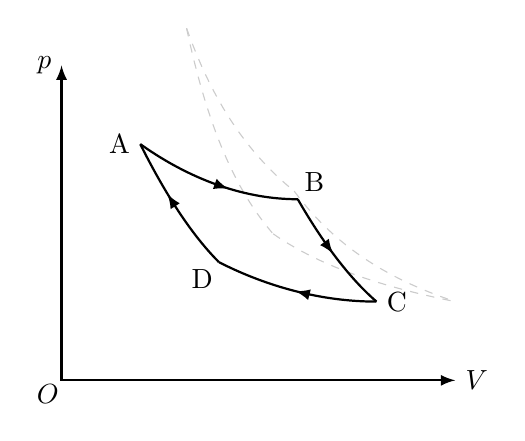
\begin{tikzpicture}
    \xOy V5p4;
    \begin{scope}[gr2, dashed]
        \draw[domain=2.6866:5]plot(\x, {5/\x});
        \draw[domain=1.5877:2.6866]plot(\x, {(3.9/\x)^(5/3)});
        \draw[domain=1.5877:2.955]plot(\x, {7.1/\x});
        \draw[domain=2.955:5]plot(\x, {(5/\x)^(5/3)});
    \end{scope}
    \draw[thick, ->-](4, 1)node[right]{C}parabola(2, 1.5)node[shift={(-135:.3)}]{D};
    \draw[thick, domain=1:2, -<-]plot(\x, {(\x-3)^2/2+1});
    \draw[thick, -<-](3, 2.3)node[shift={(45:.3)}]{B}parabola(1, 3)node[left]{A};
    \draw[thick, domain=3:4, ->-]plot(\x, {(13*(\x-5)^2+17)/30});
\end{tikzpicture}

\begin{tikzpicture}
    \xOy U4{S|_{V, n}}4;
    \draw[thick, domain=.5:3.5]plot(\x, {ln(8*\x-1)});
    \draw[dashed](1, 0)--(1, 1.946)--(3, 3.1355);
    \draw[dashed](3, 0)--(3, 3.1355);
    \draw[dashed](2, 0)--(2, 2.7);
    % \draw[dashed](0, 2.7)--(2, 2.7);
    % \draw[dashed](0, 2.54)--(2, 2.54);
    \begin{scope}[xshift=6cm]
        \xOy U4{\displaystyle\frac{\partial S}{\partial U}}4;
        \draw[thick, domain=0.5:3.5]plot(\x, {8/(8*\x-1)});
        \draw[dashed](0, 2)node[left]{$T_1^{-1}$}--(.625, 2)--(.625, 0)node[below]{$U_1$};
        \draw[dashed](0, 8/19)node[left]{$T_2^{-1}$}--(2.5, 8/19)--(2.5, 0)node[below]{$U_2$};
    \end{scope}
\end{tikzpicture}

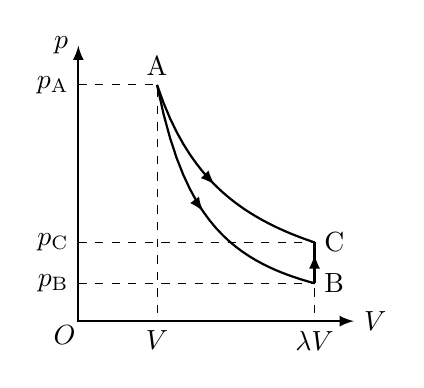
\begin{tikzpicture}
    \xOy V{3.5}p{3.5};
    \draw[thick, ->-, domain=1:3]plot(\x, {3/\x});
    \draw[thick, ->-, domain=1:3]plot(\x, {3/\x^(5/3)});
    \draw[thick](3, 1)--(3, .48);
    \draw[thick, ->](3, .48)--(3, .85);
    \draw[dashed](0, 3)node[left]{$p_{\mathrm{A}}$}--(1, 3)node[above]{A}--(1, 0)node[below]{$V$};
    \draw[dashed](0, 1)node[left]{$p_{\mathrm{C}}$}--(3, 1)node[right]{C}--(3, 0)node[below]{$\lambda V$};
    \draw[dashed](0, .48)node[left]{$p_{\mathrm{B}}$}--(3, .48)node[right]{B};
\end{tikzpicture}

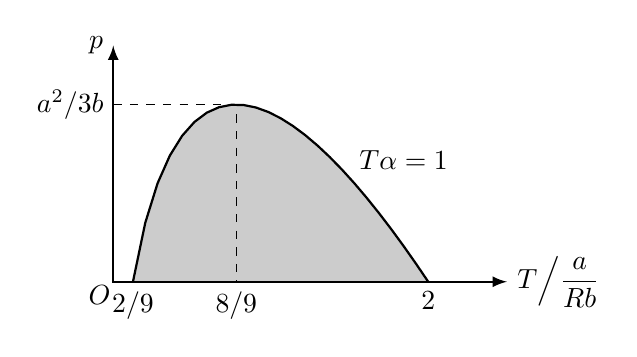
\begin{tikzpicture}
    \draw[thick, domain=.25:4, fill=cll]plot(\x, {10*sqrt(\x)-4*\x-4})node[below]{$2$};
    \xOy {T\Big/\displaystyle\frac{a}{Rb}}5p3;
    \node[below]at(1/4, 0){$2/9$};
    \node[right]at(3, 1.55){$T\alpha=1$};
    \draw[dashed](0, 9/4)node[left]{$a^2/3b$}--(25/16, 9/4)--(25/16, 0)node[below]{$8/9$};
\end{tikzpicture}

% Legendre transform
% y = (x - 1)^2/2 + 1
% p = y' = x - 1
% psi = 
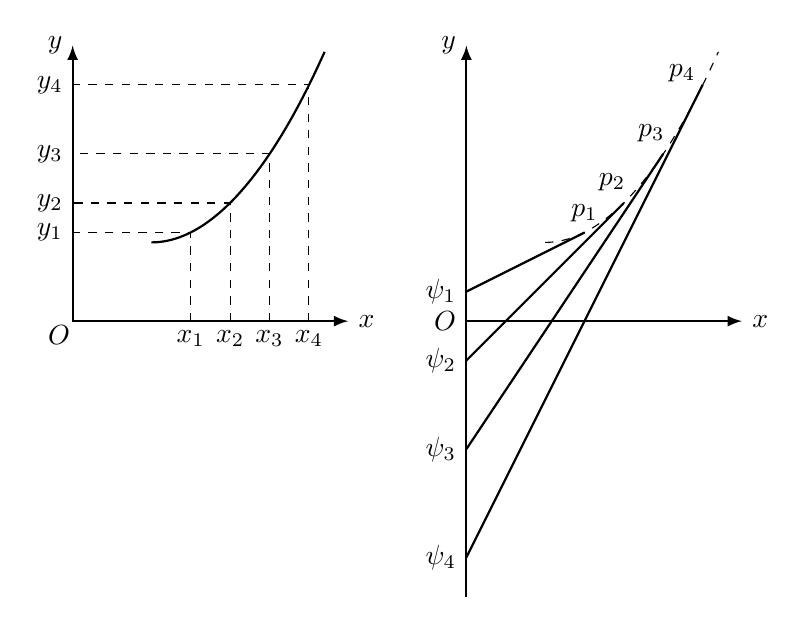
\begin{tikzpicture}
    % \fill[white](-2, -2)rectangle(10, 5);
    \xOy x{3.5}y{3.5};
    \draw[thick](1, 1)parabola(3.2, 3.42);
    \draw[dashed](1.5, 0)node[below]{$x_1$}--(1.5, 1.125)--(0, 1.125)node[left]{$y_1$};
    \draw[dashed](2, 0)node[below]{$x_2$}--(2, 1.5)--(0, 1.5)node[left]{$y_2$};
    \draw[dashed](2.5, 0)node[below]{$x_3$}--(2.5, 2.125)--(0, 2.125)node[left]{$y_3$};
    \draw[dashed](3, 0)node[below]{$x_4$}--(3, 3)--(0, 3)node[left]{$y_4$};
    \begin{scope}[xshift=5cm]
        \draw[thick, ->](0, 0)node[left]{$O$}--(3.5, 0)node[right]{$x$};
        \draw[thick, ->](0, -3.5)--(0, 3.5)node[left]{$y$};
        \draw[dashed](1, 1)parabola(3.2, 3.42);
        \draw[thick](1.5, 1.125)node[above]{$p_1$}--(0, .375)node[left]{$\psi_1$};
        \draw[thick](2, 1.5)node[shift={(120:.3)}]{$p_2$}--(0, -.5)node[left]{$\psi_2$};
        \draw[thick](2.5, 2.125)node[shift={(120:.3)}]{$p_3$}--(0, -1.625)node[left]{$\psi_3$};
        \draw[thick](3, 3)node[shift={(150:.3)}]{$p_4$}--(0, -3)node[left]{$\psi_4$};%--(5, -3)
    \end{scope}
\end{tikzpicture}

\newcommand{\hi}{_\mathrm{hi}}
\newcommand{\tot}{_\mathrm{tot}}

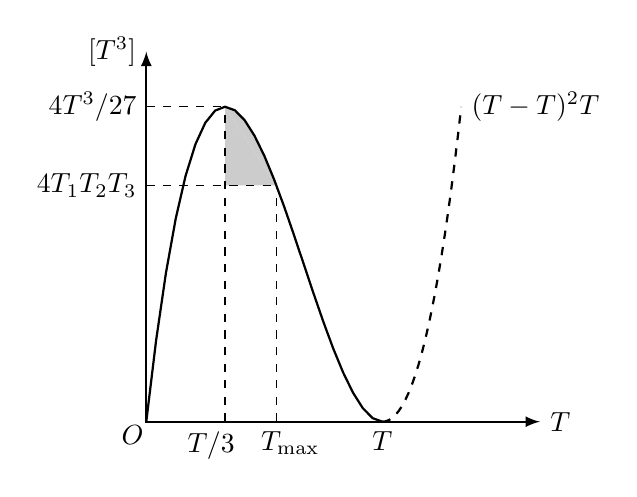
\begin{tikzpicture}
    \xOy{T\hi}{5}{[T^3]}{4.7};
    \fill[cll, domain=1:1.6527]plot(\x, {(\x-3)^2*\x});  % .468
    \fill[cll](1, 4)--(1, 3)--(1.6527, 3);
    \draw[thick, domain=0:3]plot(\x, {(\x-3)^2*\x});
    \draw[thick, domain=3:4, dashed]plot(\x, {(\x-3)^2*\x})node[right]{$(T\tot-T\hi)^2T\hi$};
    \draw[dashed](0, 3)node[left]{$4T_1T_2T_3$}--(1.6527, 3);
    \draw[dashed](0, 4)node[left]{$4T\tot^3/27$}--(1, 4);
    \draw[dashed](1, 0)node[below, xshift=-5]{$T\tot/3$}--(1, 4);
    \draw[dashed](1.6527, 0)node[below, xshift=5]{$T_\mathrm{max}$}--(1.6527, 3);
    \node at(3, 0)[below]{$T\tot$};
\end{tikzpicture}

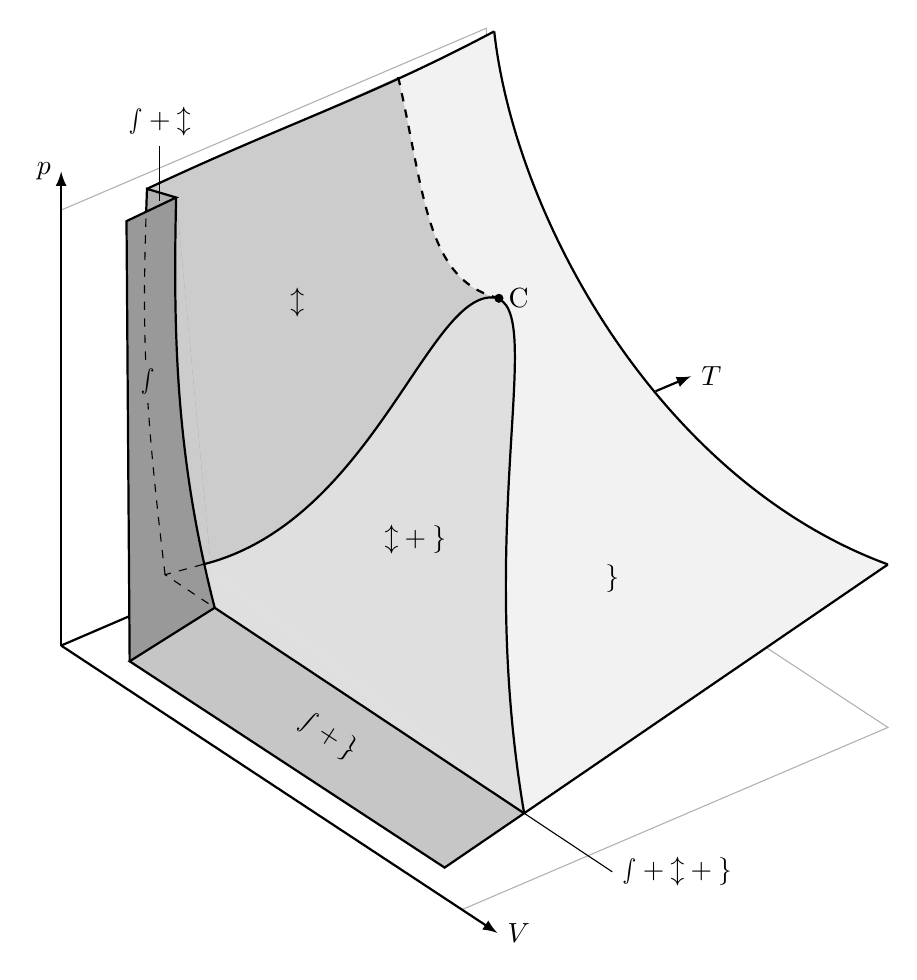
\begin{tikzpicture}
    \draw[gr3](0, 9.18)--(5.4, 11.49)--(5.4, 5.96)--(10.5, 2.61)--(5.1, 0.3);
    \draw[gr3](8, 7.07)--(5.4, 5.96)--(0.86, 4.02);
    \fill[cll](4.28, 10.87)--(5.56, 8.06)--(3, 4.7)--(1.8, 4.68)--(1.09, 9.45);
    \node at(3, 8){$\phl$};						%l
    \fill[clg](5.5, 11.45)--(4.28, 10.87)--(5.56, 8.06)--(5.5, 4)--(5.88, 1.52)--(10.5, 4.68);
    \draw[dashed, thick, fill=clg](4.28, 10.87)..controls(4.62, 9.38)and(4.63, 8.29)..(5.56, 8.06);
    \draw[thick](1.09, 9.45)..controls(2.9, 10.3)and(3.9, 10.6)..(5.5, 11.45);
    \draw[thick](5.88, 1.52)--(10.5, 4.68);
    \draw[thick, fill=white](5.5, 11.45)..controls(5.76, 9.09)and(7.59, 5.75)..(10.5, 4.68);
    \node at(7, 4.5){$\phg$};					%g
    \fill[clls](1.08, 9.16)--(1.09, 9.45)--(1.46, 9.34);
    \draw(1.25, 9.3)--(1.25, 10)node[above]{$\phs+\phl$};	%l+s
    \fill[cls](0.87, 3.45)--(1.95, 4.13)--(1.46, 9.34)--(0.83, 9.04);
    \draw[thick](1.08, 9.16)--(1.09, 9.45)--(1.46, 9.34)--(0.83, 9.04)--(0.87, 3.45);
    \fill[cll](1.95, 4.13)..controls(1.46, 6.03)and(1.42, 7.56)..(1.46, 9.34);
    \draw[dashed](1.8, 4.68)--(1.32, 4.55)--(1.95, 4.13);
    \draw[dashed](1.32, 4.55)..controls(1.05, 6.77)and(1.03, 7.64)..(1.08, 9.16);
    \node[fill=cls]at(1.1, 7){$\phs$};		%s
    \fill[clgl](1.8, 4.68)--(1.95, 4.13)--(5.88, 1.52);
    \draw[thick, fill=clgl](1.8, 4.68)..controls(3.89, 5.2)and(4.62, 7.99)..(5.43, 8.07)..controls(6.24, 8.14)and(5.23, 5.35)..(5.88, 1.52);
    \draw[thick](1.95, 4.13)..controls(1.46, 6.03)and(1.42, 7.56)..(1.46, 9.34);
    \node at(4.5, 5){$\phl+\phg$};				%g+l
    \draw[thick, fill=clsg](1.95, 4.13)--(5.88, 1.52)--(4.87, 0.83)--(0.87, 3.45)--cycle;
    \node[rotate=-33]at(3.4, 2.5){$\phs+\phg$};			%s+g
    %\draw[thick, gr4](1.95, 4.13)--(5.88, 1.52);			%s+l+g
    \draw[thick](0, 3.65)--(0.86, 4.02);
    %\draw[thick, dashed, ->](0.86, 4.02)--(5.07, 5.81);
    \draw[thick, ->](7.55, 6.88)--(8, 7.07)node[right]{$T$};
    \draw[thick, ->](0, 3.65)--(5.54, 0)node[right]{$V$};
    \draw[thick, ->](0, 3.65)--(0, 9.67)node[left]{$p$};
    \draw[fill](5.56, 8.06)circle(.05)node[right]{$\crt$};
    \draw(5.88, 1.52)--(7, .776)node[right]{$\phs+\phl+\phg$};
\end{tikzpicture}

\usetikzlibrary{calc}
\begin{tikzpicture}
    \coordinate (slend) at (1.98, 3.36);
    \coordinate (crit) at (4.31, 2.4);
    \coordinate (trip) at (2.06, 1.28);
    \fill[clg](0, 0)--(trip)--(crit)--(4.31, 3.36)--(4.9, 3.36)--(4.9, 0);
    \fill[cls](0, 0)--(trip)--(slend)--(0, 3.36);
    \fill[cll](trip)--(slend)--(4.31, 3.36)--(crit);
    %\shade[left color=lclr, right color=gclr](slend)..controls(1.14, 2.83)and(1.44, 1.95)..(trip)..controls(3.03, 1.44)and(3.71, 1.84)..(crit)--(4.31, 3.36);
    \draw[thick, fill=cls](0, 0)..controls(0.76, 0.09)and(1.56, 0.58)..(trip);
    \draw[thick, fill=cll](trip)..controls(3.03, 1.44)and(3.71, 1.84)..(crit);
    \draw[thick, fill=cll](trip)..controls(2, 1.95)and(1.98, 2.83)..(slend);
    %\draw[dashed](trip)..controls(2.34, 1.75)and(2.57, 2.47)..(2.64, 3.35);
    \draw[dashed, thick](crit)--(4.31, 3.36);
    % \draw[fill](trip)circle(.05);
    % \draw[fill](crit)circle(.05);
    \draw[thick, <->](0, 3.8)node[left]{$p$}node[right]{(log-scale)}--(0, 0)--(5.3, 0)node[right]{$T$};
    \draw let \p1=(trip) in (\x1, 0)node[below]{$T_{\mathrm{tr}}$}--(\x1, .1);
    \draw let \p2=(crit) in (\x2, 0)node[below]{$T_\crt$}--(\x2, .1);
    \node at(1, 1.6){$\phs$};
    \node at(3.3, .8){$\phg$};
    \node at(3, 2.6){$\phl$};
\end{tikzpicture}

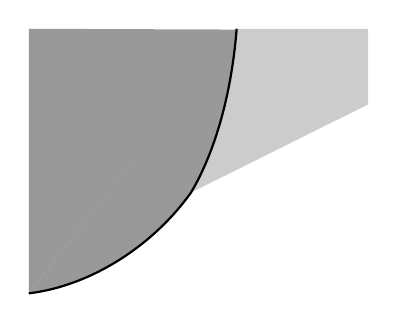
\begin{tikzpicture}
    \fill[cls](0, 0)--(2.64, 3.35)--(0, 3.36);
    \fill[cll](2.06, 1.28)--(2.64, 3.36)--(4.31, 3.36)--(4.31, 2.4);
    \draw[thick, fill=cls](0, 0)..controls(0.76, 0.09)and(1.56, 0.58)..(2.06, 1.28)..controls(2.34, 1.75)and(2.57, 2.47)..(2.64, 3.36);
\end{tikzpicture}

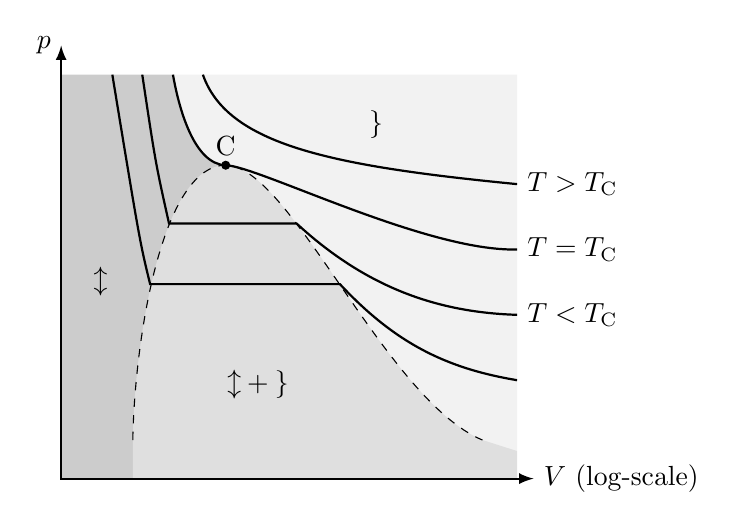
\begin{tikzpicture}
    \fill[cll](0, 0)--(0, 5.13)--(1.42, 5.13)--(2.09, 3.98)--(0.91, 0);
    \fill[clg](1.42, 5.13)--(2.09, 3.98)--(3, .35)--(5.79, .35)--(5.79, 5.13);
    \fill[clgl](0.91, 0)--(0.91, .49)--(5.35, .49)--(5.79, 0.35)--(5.79, 0);
    \draw[dashed, fill=clgl](0.91, 0.49)..controls(0.93, 1.72)and(1.27, 3.98)..(2.09, 3.98)..controls(2.91, 3.98)and(4.11, 1.01)..(5.35, 0.49);
    \draw[thick](0.65, 5.13)..controls(1, 3)..(1.13, 2.47)--(3.54, 2.47)..controls(4.24, 1.72)and(4.89, 1.4)..(5.79, 1.25);
    \draw[thick](1.03, 5.13)..controls(1.2, 4)..(1.37, 3.24)--(2.99, 3.24)..controls(3.9, 2.4)and(4.82, 2.11)..(5.79, 2.08)node[right]{$T<T_\crt$};
    \draw[thick, fill=clg](1.42, 5.13)..controls(1.49, 4.73)and(1.68, 3.99)..(2.09, 3.98)..controls(2.5, 3.97)and(4.64, 2.88)..(5.79, 2.91)node[right]{$T=T_\crt$};
    \draw[thick](1.8, 5.13)..controls(2.11, 4.24)and(3.43, 3.97)..(5.79, 3.74)node[right]{$T>T_\crt$};
    %\node[right]at(5.79, 4.57){$T\gg T_\crt$};
    \draw[thick, <->](0, 5.5)node[left]{$p$}--(0, 0)--(6, 0)node[right]{$V$ (log-scale)};
    \draw[fill](2.09, 3.98)circle(.05)node[above]{C};
    \node at(.5, 2.5){$\phl$};
    \node at(2.5, 1.2){$\phl+\phg$};
    \node at(4, 4.5){$\phg$};
\end{tikzpicture}

\begin{tikzpicture}
    \xOy T4p4;
    \draw[thick](1, 1)..controls(1.6, 1.1)and(2.8, 2.5)..(3, 3);
    \draw[fill](3, 3)circle(.05)node[right]{$\crt$};
    \node at(1.5, 2.8){$\phl$};
    \node at(3, 1.3){$\phg$};
\end{tikzpicture}

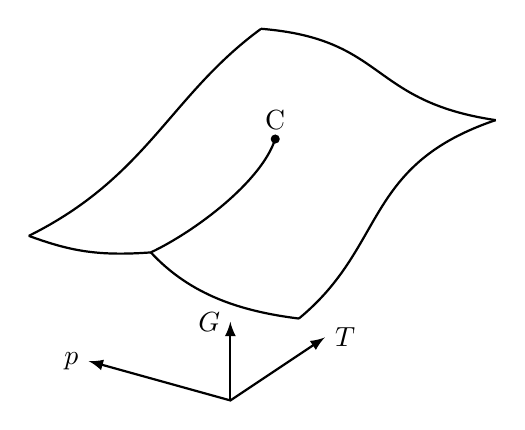
\begin{tikzpicture}
    \draw[thick](0.24, 2.09)..controls(0.76, 1.9)and(1.11, 1.83)..(1.79, 1.88);
    \draw[thick](1.79, 1.88)..controls(2.3, 1.33)and(2.95, 1.13)..(3.67, 1.04);
    \draw[thick](1.79, 1.88)..controls(2.34, 2.14)and(3.19, 2.77)..(3.37, 3.32);
    \draw[thick](0.24, 2.09)..controls(1.75, 2.84)and(2.03, 3.87)..(3.19, 4.72);
    \draw[thick](3.67, 1.04)..controls(4.79, 1.96)and(4.48, 2.99)..(6.17, 3.56);
    \draw[thick](3.19, 4.72)..controls(4.79, 4.59)and(4.55, 3.8)..(6.17, 3.56);
    \draw[fill](3.37, 3.32)circle(.05)node[above]{$\crt$};
    \draw[thick, <-](2.8, 1)node[left]{$G$}--(2.8, 0);
    \draw[thick, <->](1, .5)node[left]{$p$}--(2.8, 0)--(4, .8)node[right]{$T$};
\end{tikzpicture}

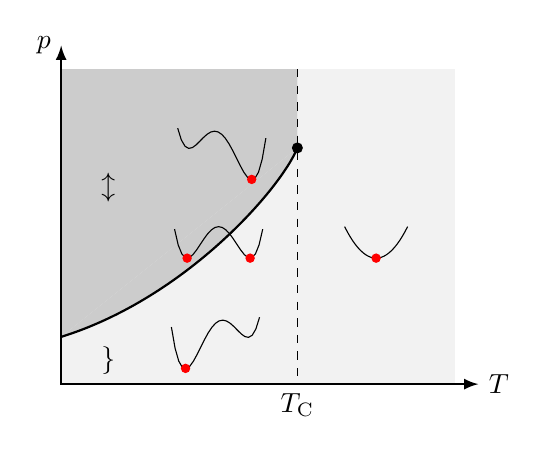
\begin{tikzpicture}
    \fill[clg](0, 0)--(0, .6)--(3, 3)--(3, 4)--(5, 4)--(5, 0);
    \fill[cll](0, .6)--(0, 4)--(3, 4)--(3, 3);
    \draw[thick, fill=cll](0, 0.6)..controls(1.6, 1.1)and(2.8, 2.5)..(3, 3);
    \fill(3, 3)circle(.07);
    \draw[thick, <->](5.3, 0)node[right]{$T$}--(0, 0)--(0, 4.3)node[left]{$p$};
    \draw[dashed](3, 4)--(3, 0)node[below]{$T_\crt$};
    \node at(.6, .3){$\phg$};
    \node at(.6, 2.5){$\phl$};
    \begin{scope}[scale=0.4, xshift=5cm]
        \begin{scope}[yshift=2cm]
            \draw[domain=-1.5:1.3]plot(\x, {(\x)^4-2*(\x)^2+\x/2});
            \fill[red](-1.05, -1.5)circle(.15);
        \end{scope}
        \begin{scope}[yshift=5cm]
            \draw[domain=-1.4:1.4]plot(\x, {(\x)^4-2*(\x)^2});
            \fill[red](-1, -1)circle(.15);
            \fill[red](1, -1)circle(.15);
        \end{scope}
        \begin{scope}[yshift=8cm]
            \draw[domain=-1.3:1.5]plot(\x, {(\x)^4-2*(\x)^2-\x/2});
            \fill[red](1.05, -1.5)circle(.15);
        \end{scope}
        \begin{scope}[shift={(5, 4)}]
            \draw[domain=-1:1]plot(\x, {(\x)^2});
            \fill[red](0, 0)circle(.15);
        \end{scope}
    \end{scope}
\end{tikzpicture}

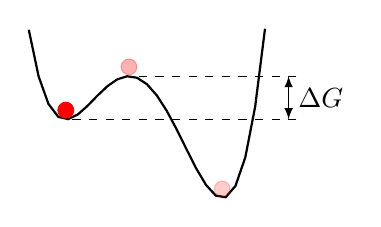
\begin{tikzpicture}
    \draw[thick, domain=-1.4:1.6]plot(\x, {(\x)^4-2*(\x)^2-\x/2});
    \draw[fill, red](-.93, -.4)circle(.1);
    \draw[fill, red, opacity=.3](-.127, .15)circle(.1);
    \draw[fill, red, opacity=.2](1.057, -1.4)circle(.1);
    \draw[dashed](2, -.516)--(-.93, -.516);
    \draw[dashed](2, .032)--(-.127, .032);
    \draw[<->](1.9, -.516)--(1.9, .032)node[midway, right]{$\Delta G$};
    %\draw(1.057, -1.515)--(-1, -1.515);
\end{tikzpicture}

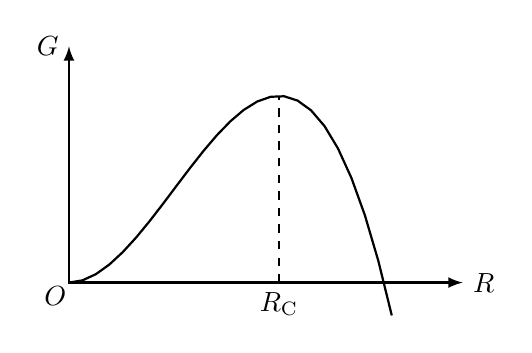
\begin{tikzpicture}[scale=2]
    \xOy R{2.5}G{1.5};
    \draw[thick, domain=0:2.05]plot(\x, {2*(\x)^2-(\x)^3});
    \draw[dashed](4/3, 0)node[below]{$R_\crt$}--(4/3, 32/27);
\end{tikzpicture}

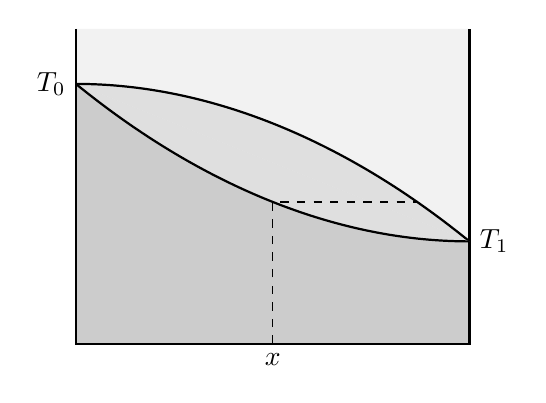
\begin{tikzpicture}
    \fill[cll](0, 0)--(5, 0)--(5, 1.3)--(0, 3.3);
    \fill[clg](0, 4)--(5, 4)--(5, 1.3)--(0, 3.3);
    \draw[thick](0, 4)--(0, 0)--(5, 0)node[midway, below]{$x$}--(5, 4);
    \draw[thick, fill=clgl](0, 3.3)parabola(5, 1.3)node[right]{$T_1$};
    \draw[thick, fill=clgl](5, 1.3)parabola(0, 3.3)node[left]{$T_0$};
    \draw[dashed](2.5, 0)--(2.5, 1.8)--(4.33, 1.8);
\end{tikzpicture}

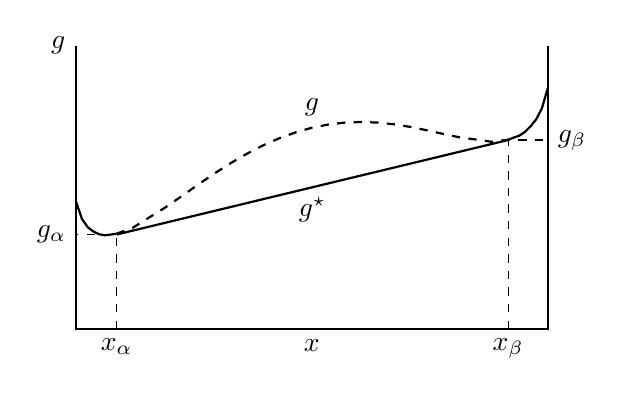
\begin{tikzpicture}[scale=6]
    \draw[thick](0, .6)node[left]{$g$}--(0, 0)--(1, 0)node[midway, below]{$x$}--(1, .6);
    \draw[thick, domain=.001:.0867, samples=8]plot(\x, {4*(-(\x-.53)^2+.7)+1.4*(\x*ln(\x)+(1-\x)*ln(1-\x))-1.4});
    \draw[thick, dashed, domain=.0867:.91532]plot(\x, {4*(-(\x-.53)^2+.7)+1.4*(\x*ln(\x)+(1-\x)*ln(1-\x))-1.4});
    \node at(.5, .47){$g$};
    \draw[thick, domain=.91532:.999, samples=8]plot(\x, {4*(-(\x-.53)^2+.7)+1.4*(\x*ln(\x)+(1-\x)*ln(1-\x))-1.4});
    \draw[thick](.0867, .2)--(.91532, .4)node[midway, below]{$g^\star$};
    \draw[dashed](.0867, 0)node[below]{$x_\alpha$}--(.0867, .2)--(0, .2)node[left]{$g_\alpha$};
    \draw[dashed](.91532, 0)node[below]{$x_\beta$}--(.91532, .4)--(1, .4)node[right]{$g_\beta$};
\end{tikzpicture}

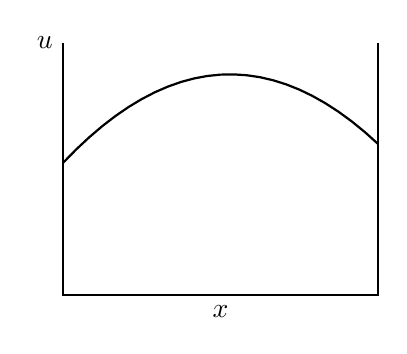
\begin{tikzpicture}[scale=4]
    \draw[thick](0, .8)node[left]{$u$}--(0, 0)--(1, 0)node[midway, below]{$x$}--(1, .8);
    \draw[thick, domain=0:1]plot(\x, {-(\x-.53)^2+.7});
\end{tikzpicture}

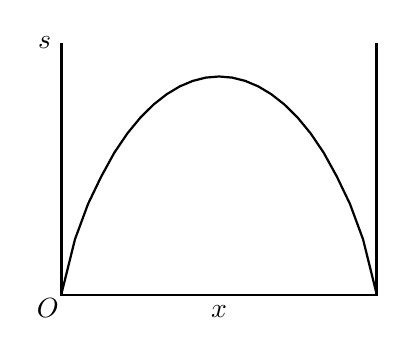
\begin{tikzpicture}[scale=4]
    \draw[thick](0, .8)node[left]{$s$}--(0, 0)node[shift={(-135:7pt)}]{$O$}--(1, 0)node[midway, below]{$x$}--(1, .8);
    \draw[thick, domain=.001:.999]plot(\x, {-\x*ln(\x)-(1-\x)*ln(1-\x)});
\end{tikzpicture}

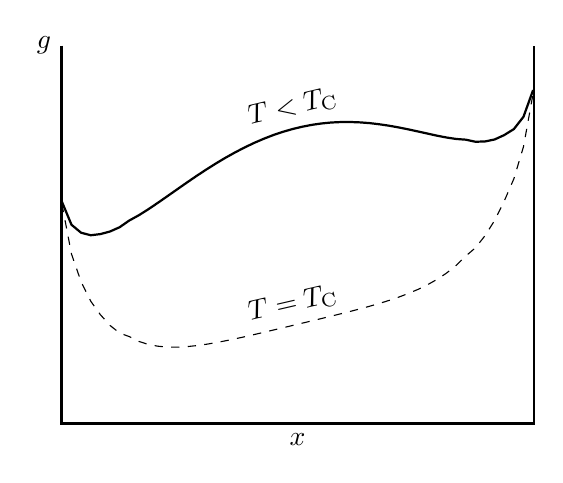
\begin{tikzpicture}[scale=6]
    \draw[thick](0, .8)node[left]{$g$}--(0, 0)--(1, 0)node[midway, below]{$x$}--(1, .8);
    \draw[thick, domain=.001:.999, samples=50]plot(\x, {4*(-(\x-.53)^2+.7)+1.4*(\x*ln(\x)+(1-\x)*ln(1-\x))-1.2});
    \node[above, rotate=13.5]at(.5, .626){$T<T_\crt$};
    \draw[dashed, domain=.001:.999, samples=50]plot(\x, {4*(-(\x-.53)^2+.7)+2*(\x*ln(\x)+(1-\x)*ln(1-\x))-1.2});
    \node[above, rotate=13]at(.5, .21){$T=T_\crt$};
\end{tikzpicture}

\begin{tikzpicture}
    \draw[thick, ->](0, 0)node[left]{$O$}--(4.5, 0)node[right]{$N_+$};
    \draw[thick, ->](0, -2.5)--(0, 2.5)node[left]{$T$};
    % \node[shift={(-135:9pt)}]at(0, 0){$O$};
    \draw[thick, domain=.001:1.77]plot(\x, {.5/ln((4-\x)/\x)});
    \draw[thick, domain=2.23:3.999]plot(\x, {.5/ln((4-\x)/\x)});
    \draw[dashed](2, -2.5)--(2, 2.5);
    \draw[thick](4, 0)node[above]{$N$}--(4, -.06);
\end{tikzpicture}

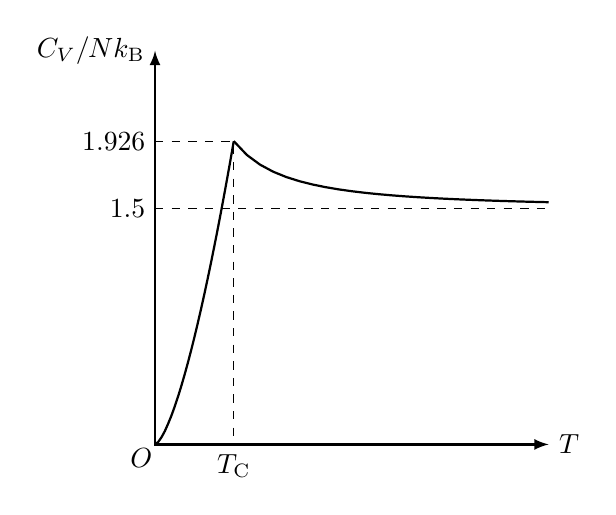
\begin{tikzpicture}[yscale=2]
    \xOy T5{C_V/N\kB}{2.5};
    \draw[dashed](0, 1.926)node[left]{1.926}--(1, 1.926)--(1, 0)node[below]{$T_\crt$};
    \draw[dashed](0, 1.5)node[left]{1.5}--(5, 1.5);
    \draw[thick, domain=0:1]plot(\x, {1.926 * \x^1.5});
    \draw[thick, domain=1:5]plot(\x, {1.5 + (1.926-1.5)/(\x^1.5)});
\end{tikzpicture}

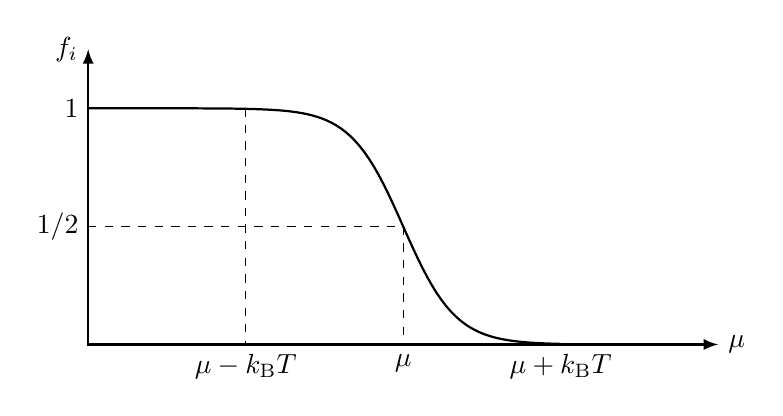
\begin{tikzpicture}[xscale=2, yscale=1.5]
    \draw[thick, <->](4, 0)node[right]{$\mu$}--(0, 0)--(0, 2.5)node[left]{$f_i$};
    \node[left]at(0, 2){1};
    \draw[dashed](0, 1)node[left]{$1/2$}--(2, 1)--(2, 0)node[below]{$\mu$};
    \draw[dashed](1, 2)--(1, 0)node[below]{$\mu-\kB T$};
    \node[below]at(3, 0){$\mu+\kB T$};
    \draw[thick, domain=0:3, samples=100]plot(\x, {2 / (1 + exp(6*\x-12))});
\end{tikzpicture}

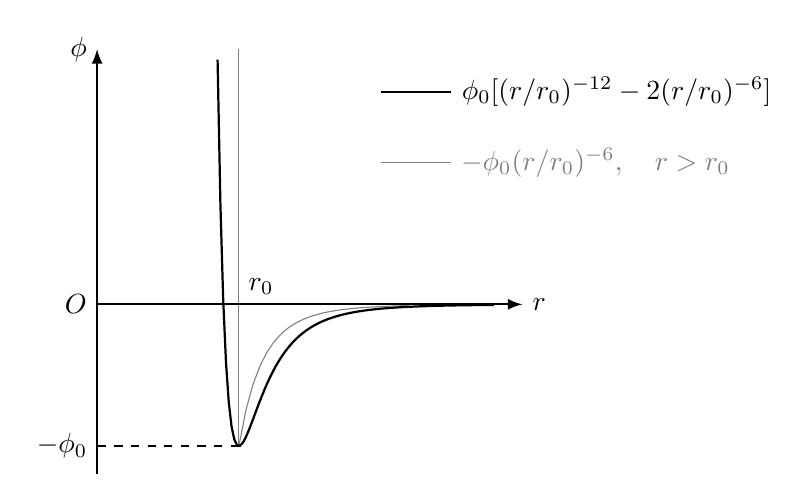
\begin{tikzpicture}[scale=1.8]
    \draw[gray](1, 1.8)--(1, -1);
    \draw[gray, domain=1:2.2]plot(\x, {-\x^(-6)});
    \draw[thick, ->](0, 0)node[left]{$O$}--(3, 0)node[right]{$r$};
    \draw[thick, ->](0, -1.2)--(0, 1.8)node[left]{$\phi$};
    \draw[dashed](1, -1)--(0, -1)node[left]{$-\phi_0$};
    \node[above right]at(1, 0){$r_0$};
    \draw[thick, domain=.85:2.8, samples=100]plot(\x, {\x^(-12)-2*\x^(-6)});
    \draw[thick, shift={(2, 1.5)}](0, 0)--(.5, 0)node[right]{$\phi_0[(r/r_0)^{-12}-2(r/r_0)^{-6}]$};
    \draw[gray, shift={(2, 1)}](0, 0)--(.5, 0)node[right]{$-\phi_0(r/r_0)^{-6},\quad r>r_0$};
\end{tikzpicture}

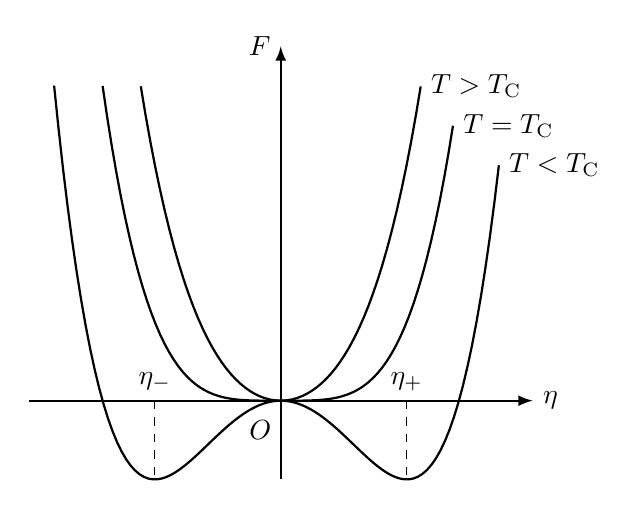
\begin{tikzpicture}[xscale=1.6]
    \node[shift={(-125:.45)}]at(0, 0){$O$};
    \draw[thick, ->](-2, 0)--(2, 0)node[right]{$\eta$};
    \draw[thick, ->](0, -1)--(0, 4.5)node[left]{$F$};
    \draw[thick, domain=-1.111:1.111, samples=60]plot(\x, {(\x)^4+2*(\x)^2})node[right]{$T>T_\crt$};
    \draw[thick, domain=-1.414:1.368, samples=80]plot(\x, {(\x)^4})node[right]{$T=T_\crt$};
    \draw[thick, domain=-1.799:1.732, samples=100]plot(\x, {(\x)^4-2*(\x)^2})node[right]{$T<T_\crt$};
    \draw[dashed](1, 0)node[above]{$\eta_+$}--(1, -1);
    \draw[dashed](-1, 0)node[above]{$\eta_-$}--(-1, -1);
\end{tikzpicture}

\end{document}